\documentclass[10pt,letterpaper,twocolumn]{article}

%2012-10-01 - Document préparé par David Lafrenière, pour le cours PHY3040.

%Pour langue et caractères spéciaux
%en français svp
\usepackage[francais]{babel}
\usepackage[utf8]{inputenc}  
\usepackage[T1]{fontenc} 

\usepackage{amssymb}
\usepackage{amsmath}
\usepackage{mathrsfs}
%(dé)commenter la bonne ligne de ce qui suit selon votre système d'opération
%\usepackage[applemac]{inputenc} %pour MAC OS X, enlever le "%" en début de ligne si votre système est un MAC
%\usepackage[ansinew]{inputenc} %pour Windows, enlever le "%" en début de ligne si votre système est sous Windows

%Pour ajuster les marges
\usepackage[top=2cm, bottom=2cm, left=2cm, right=2cm, columnsep=20pt]{geometry}

%chez nous
\newcommand{\folder}{/home/eric/UdeM/session_5/Lab3/template}

%laptop
%\newcommand{\folder}{/home/delta137/Documents/lab3}
%share_latex
%\newcommand{\folder}{}
% Pour la commande onecolabstract (résumé 1 pleine largeur)
\usepackage{\folder/abstract}
	\renewcommand{\abstractnamefont}{\normalfont\bfseries}
	\renewcommand{\abstracttextfont}{\normalfont\itshape}

% Pour les titres de section/sous-section
\usepackage[compact]{\folder/titlesec}
\titleformat{\section}{\large\bfseries}{\thesection}{1em}{}
\titleformat{\subsection}{\normalsize\bfseries}{\thesubsection}{1em}{}
\titleformat{\subsubsection}{\normalsize}{\thesubsubsection}{1em}{}


%pour inclure des graphiques
\usepackage{\folder/graphicx}

%pour tableaux deluxetable
\usepackage{\folder/deluxetable}

%Pour inclure des adresse web
\usepackage{\folder/url}

%Titre
\title{\vspace{-10mm}\Large
Optique non-linéaire
\vspace{-4mm}}

%Auteur
\author{\large
Éric Dupuis\\
}
\date{\vspace{-8mm}}

\begin{document}

\twocolumn[
\maketitle
\begin{onecolabstract}
%***remplacer le texte qui suit par votre résumé***
\noindent La formation d'un laser vert  a été tentée dans le but d'explorer et caractériser plusieurs principes d'optique non-linéaire. Une faisceau avec $\lambda= 1064 \,nm$ a été formé par inversion de population en excitant à 808 nm un cristal de ND:YV$O_4$. La longueur optimale de la cavité optique est de $13.0\pm 0.1 \,cm$. Une augmentation linéaire du rapport de la raie émise (1064 nm) par rapport à la raie d'excitation (808 nm) en fonction de l'intensité du faisceau incident a été observée. Le spectre d'émission spontanée du ND:YV$O_4$ a montré la présence d'autre raies d'émission à 914 et XXX nm. La génération d'une raie à 532 nm avec un cristal de KTP n'a pas été réussie. La fluorescence  dans la rhodanine excitée à 532 nm par un autre laser a montré un déplacement de Stokes de XX nm.
\vspace{4mm} %
\end{onecolabstract}
]

%***à partir d'ici, éditer à votre guise***
\section{Introduction}\label{intro}
%L'apport de la physique fondamentale à la technologique moderne est essentiel,
La nature recèle de nombreux processus très utiles pour autant qu'on sache catalyser leur effet.  
%Notre connaissance de la nature améliore notre contrôle sur des phénomènes utiles.
% Mieux la nature est comprise, plus ses phénomènes peuvent être exploités dams pour la société. Les lasers    En particulier, 
Par exemple, la stimulation d'un électron par un photon peut mener à la radiation cohérente de deux photons. En laboratoire, ce processus est décuplé par une inversion de population, permettant la formation d'un laser, un outil aux applications très variées. Dans ce contexte, on voudra étudier les étapes successives qui produisent ensemble un laser vert en partant d'une source cohérente de lumière à longueur d'ondes ($\lambda$) de 808 nm. La présence de niveaux d'énergie métastables dans un cristal de  Nd:YV$O_4$  et le doublage de fréquence par la polarisation des atomes dans un cristal KTP seront exploités afin de modifier la longueur d'ondes du faisceau initial. On se servira du laser produit pour induire la fluorescence dans le rhobodamine B et on y observera le déplacement de Stokes. 

\section{Théorie}
%inversion de population
Les couches électroniques dans les atomes donnent accès à des niveaux d'énergies différentes. Un électron qui absorbe ou émet un photon va respectivement monter ou descendre de niveau d'énergie. Il peut également absorber un photon, puis en émettre deux qui gardent la polarisation et la phase du photon incident. On parle alors d'émission stimulée. Moyennant plusieurs électrons dans un niveau d'énergie supérieur et une cavité optique permettant de confiner les photons émis, on peut bâtir un faisceau cohérent, un laser. \\

À température de la pièce, les électrons des atomes d'un matériel occupent majoritairement l'état de base. Une source cohérente de lumière peut pomper les électrons vers un état d'énergie supérieure. L'émission stimulée est typiquement marginale vu le temps de vie très court du niveau. Par contre, la présence d'un niveau métastable inférieur au niveau excité permet d'accumuler des électrons dans un niveau supérieur à l'état de base. Si le taux de pompage est supérieur au taux d'émission spontanée, l'état métastable devient plus peuplé que l'état de base. Cette inversion de population augmente la probabilité d'émission stimulée. Une cavité optique permet de conserver les photons cohérents et d'augmenter graduellement leur nombre jusqu'à l'atteinte d'un équilibre.\\

L'émission cohérente à partir du niveau métastable produit un nouveau faisceau distinct du premier assurant le pompage des électrons du niveau de base. La polarisation d'un matériau par le faisceau peut aussi produire une longueur d'onde distincte. Étant donné un milieu non-linéaire qui ne présente pas de symétrie d'inversion, une polarisation au deuxième ordre est possible et oscille à la seconde harmonique du faisceau incident. À condition d'offrir une longueur de cohérence satisfaisante avec la première harmonique, une onde allant comme la seconde harmonique est effectivement créée.\\

La fluorescence est le phénomène de réémission spontanée et directe d'une molécule, souvent excitée par l'absorption d'un photon. Dans les matériaux fluorescents,  une partie de l'énergie transmise par l'excitation est perdue en énergie vibrationnelle. Il en résulte des photons d'une longueur d'onde plus grande. L'effet de décalage du spectre d'émission par rapport au spectre d'absorption ainsi causé est appelé déplacement de Stokes.\\


%  une polarisation aux ordres supérieurs est générée par la seconde harmonique du faisceau incident. peut générer une polarisation, aux ordres supérieurs,  



 % et de favoriserlargement défavorisée Le taux de désintégration dans le sens inverse  , le temps de vie des niveaux excités est trop faible. La présence de niveaux d'énergie  Un matériel Pour favoriser l'émission stimulée, il faut d'abord  La migration forcée
%expliquer diode
\section{Méthodologie et prise de données}\label{sec:eq}

\subsection{Montage et manipulations}
La figure \ref{fig:schéma} montre un schéma du montage expérimental. Une diode-laser émet des photons de $\lambda = 808 \, \text{nm}$ qui sont focalisés par une lentille à gradient d'indice (GRIN) dans un cristal de Nd:YV$O_4$. Le cristal est positionné à environ 2 cm de la lentille . La source de photons pompe les électrons dans l'état de base du cristal vers un niveau supérieur. Un niveau métastable peuplé par le pompage favorise l'émission  stimulée de photons à $\lambda = 1064 \,\text{nm}$. Le cristal est placé dans un milieu de gain borné par un miroir et la lentille (aussi un miroir). Le miroir, semi-perméable, permet à la fois le confinement des photons et la sorie du faisceau cohérent. Celui-ci  est acheminé à un spectromètre par une fibre optique dans l'axe optique.
\textbf{\begin{figure}[ht]
\centering
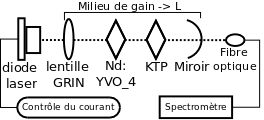
\includegraphics[width=1\linewidth]{schem1.png}
\caption{\label{fig:schéma} Table d'optique. $L$ est la longueur du milieu de gain qui est borné par la lentille et le miroir. Une première étude est réalisée sans le KTP.}
\end{figure}}

La distance relative et l'orientation des éléments  dans le milieu de gain est d'abord optimisée, le trajet optique est vérifié par un laser rouge.  Dans une première étude qui n'inclut pas encore le cristal KTP, la longueur $L$ du milieu de gain est variée par le changement de position du miroir. L'amplitude relative du pic à $\lambda= 1064 \, \text{nm}$ est comparée à celle du faisceau original à $\lambda = 808 \, \text{nm}$ en fonction de $L$. On fait la même étude, cette fois en fonction de l'intensité du faisceau, donc de la puissance envoyée  à la diode laser par le contrôle du courant.\\

Dans un deuxième temps, un cristal de KTP est ajouté et sert de milieu non-linéaire où la seconde harmonique est générée. La bi-réfringence du cristal permet, en dépit de la dispersion, de maintenir la phase entre la première et la seconde harmonique. Vu l'importance de la direction dans ce cristal, son orientation peut être modifiée relativement à la plaque qui le contient. La sensibilité du faisceau à la direction du cristal KTP explique pourquoi l'alignement relatif des deux cristaux est l'un des points critiques. Cette fois, les mesures prévues étaient les amplitudes relatives des pics à 532, 808 et 1064 nm sont prises en fonction de la postion du miroir, de la puissance dans la diode et de l'orientation du KTP.\\

Dans la dernière partie, un filtre à l'extérieur du milieu de gain est placé pour isoler la raie de 532 nm. Des solutions de concentration 1mM de Rhodamine B dans l'eau et l'octanol sont mises dans une cuvette de 1 cm de longueur dans l'axe optique. On leur dirige le faisceau vert, Le spectromètre placé hors de l'axe  capte le spectre d'émission des solutions. \\

\subsection{Mesures et incertitudes}
Chaque partie de l'expérience tente de caractériser la réponse du spectromètre à la variation de paramètres du montage optique. Les incertitudes qui caractérisent la position du miroir sur le banc d'optique $\pm 0.1 cm$, l'intensité envoyée dans la diode $\pm 1 mA$ et l'orientation du cristal KTP $\pm 0.1 \deg???$ sont et petites relativement à la grandeur de leur mesure. Quant à elle, la réponse du spectre est toujours légèrement instable. L'  incertitude relative de l'intensité des raies est toujours au moins d'environ 2\%. Donc, l'incertitude sur le rapport des amplitudes des raies est d'autant plus important et domine généralement les autres incertitudes.\\

De plus, pour calculer le rapport des amplitudes des pics d'émission, on doit d'abord soustraire à l'intensité des raies la mesure du fond limuneux ambiant. La raie de 1064 nm présentait souvent de grandes fluctuations que nous avons négligées et interprétées comme une instabilité du montage. Nous avons gardé les petites fluctuations autour du maximum pour évaluer l'incertitude sur l'amplitude de la raie. \\ 

Étant donné que la raie de 808 nm a une amplitude beaucoup plus grande que la raie 1064 nm dans l'axe optique, les temps d'intégration qui rendent la raie de 1064 nm observable saturent la raie à 808 nm. Pour mesurer l'intensité de la raie de 808 nm, on doit appliquer un filtre de densité neutre que l'on place directement devant la fibre optique. Un facteur de réduction a été mesuré pour plusieurs puissances dans la diode. \\

Pour ce faire, l'intensité de la raie à 808 nm a été mesurée avant et après filtrage. Le facteur a été obtenu pour des puissances entre  150 et 400 mA; Pour les puissances plus hautes, la raie originale était saturée même pour le plus petits temps d'intégration.  Dans ces cas, il fallait éloigner le spectromètre  de la source pour diminuer le flux. Nous avons vérifié que la distance du filtre par rapport au spectromètre n'affectait pas la réduction. Nous avons trouvé un facteur moyen de réduction de $30 \pm 6$. %C'est dû à une mesure à 400 mA plus basse que les autres. Cependant, l'incertitude de chaque facteur pour les différentes puissances est de l'ordre de 6.  
Comme on évitait la saturation de la raie non filtrée, on travaillait à petit temps d'intégration et l'intensité de la raie filtrée avait une grande incertitude relative. Ceci explique la grande incertitude sur le facteur de réduction. Une seule puissance a donné un facteur s'éloignant de plus d'un écart-type de la moyenne, nous avons conclu que le facteur de réduction était constant. Avec cette conclusion, on peut simplement comparer les données brutes entre elles sans avoir à appliquer le facteur de réduction, même lorsque la puissance est variée.

%Au final, le facteur de réduction était plutôt constant. nous avons trouvé un facteur de réduction plutôt constant pour les différentes La figure \ref{fig:calib} montre que le facteur tend à diminuer de façon assez linéaire en fonction de la puissance dans la diode. La relation  $F_r = xP_d$ est trouvée et utilisée pour convertir les mesures d'amplitude de la raie à 808 nm.  Dans certains  \\

%\textbf{\begin{figure}[ht]
%\centering
%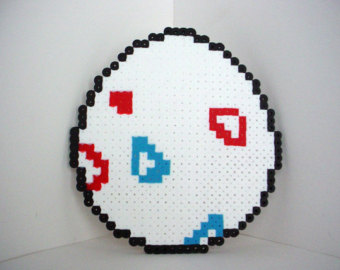
\includegraphics[width=0.1\linewidth]{\folder/wip.jpg}
%\caption{\label{fig:calib} Facteur de réduction $F_r$ du filtre de densité neutre en fonction de la puissance $P_d$ envoyée dans la diode. Une régression linéaire donne la relation $F_r = xP_d$}
%\end{figure}}

En raison des difficultés à bien aligner les deux cristaux dans la deuxième partie, une série de mesures à été réalisée pour mieux caractériser le faisceau de 1064 nm. En particulier, le spectre d'émission spontanée a été étudié. L'absorption dans  la rhodanine B   des raies de longueurs d'ondes 808 nm et 1064 nm a aussi été investigué. 
 
\subsection{Résultats et analyse}

Les équations peuvent être insérées directement dans le texte en les écrivant entre deux signes de dollar (\$). Par exemple,  \verb|$n_1 \cos{\theta_1}=n_2 \cos{\theta_2}$| donnera ceci: $n_1 \cos{\theta_1}=n_2 \cos{\theta_2}$. Dans ce cas, l'équation n'est pas numérotée.

\subsection{Équations sur une ligne à part}

Les équations peuvent aussi occuper leur propre ligne, en utilisant \verb|\begin{equation}| et \verb|\end{equation}|. Voici un exemple:

\begin{equation}\label{eq1}
n_1 \cos{\theta_1}=n_2 \cos{\theta_2}.
\end{equation}

\noindent Dans ce cas, elles sont numérotées automatiquement. Comme pour les sections, on peut référer à l'équation \ref{eq1} en utilisant la commande \verb|\ref{}| en combinaison avec la commande \verb|\label{}|.

\section{Figures}

Un graphique peut être inséré à l'aide de la commande \verb+includegraphics{}+. Cette commande comporte quelques options pour ajuster la taille ou l'orientation de l'image, en voici quelques exemples:
\begin{verbatim}
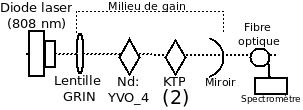
\includegraphics{schem1.jpeg}
\includegraphics[height=60mm]{fig.jpg}
\includegraphics[width=0.8\linewidth]{fig.png}
\includegraphics[scale=0.75]{fig.pdf}
\includegraphics[angle=45]{fig.pdf}
\end{verbatim}

Selon le compilateur utilisé, {\em pdflatex} ou {\em latex}, seulement quelques formats de fichiers graphiques peuvent être insérés. Avec le compilateur {\em pdflatex}, seulement les formats PDF, PNG, et JPEG sont supportés, alors qu'avec le compilateur {\em latex}, seulement le format PS (ou EPS) est supporté. Pour être correctement numérotées et bien positionnées, les figures doivent être insérées dans l'environnement {\em figure}, avec les commandes \verb+\begin{figure}+ et \verb+\end{figure}+, comme dans l'exemple qui suit:
\begin{verbatim}
\begin{figure}[ht]
\centering

\includegraphics[width=0.7\linewidth]{\folder/logo}
\caption{\label{fig:logo} Logo de 
l'Université de Montréal.}
\end{figure}
\end{verbatim}



\begin{figure*}[t]
\centering

\includegraphics[width=0.8\textwidth]{\folder/logo}
\caption{\label{fig:logo2} Logo de l'Université de Montréal.}
\end{figure*}

Ceci donne le résultat montré à la figure \ref{fig:logo}, où la figure apparaît sur une seule colonne. Pour insérer une figure qui s'étend en largeur sur les deux colonnes, il faut plutôt utiliser l'environnement {\em figure*}, avec les commandes \verb+\begin{figure*}+ et \verb+\end{figure*}+. Un tel exemple est montré à la figure~\ref{fig:logo2}. La description de la figure est ajoutée à l'aide de la commande \verb+\caption{}+, laquelle doit être placée à l'intérieur de l'environnement {\em figure}.

Comme pour les sections et les équations, on peut référer à une figure donnée en utilisant la commande \verb|\ref{}| en combinaison avec la commande \verb|\label{}|.

\section{Tableaux}

De façon similaire aux figures, il faut placer les tableaux dans l'environnement {\em table}, avec les commandes \verb+\begin{table}+ et \verb+\end{table}+. Ensuite, à l'intérieur de cet environnement on doit entrer dans un autre environnement, {\em tabular}, avec les commandes \verb+\begin{tabular}+ et \verb+\end{tabular}+. C'est à l'intérieur de l'environnement {\em tabular} que l'on construit la table. Par exemple, le code suivant donne le résultat montré à la table~\ref{tab}.
\begin{verbatim}
\begin{table}[th]
\label{tab}
\centering
\begin{tabular}{ l | c | c }
   & $I_{\rm max}$ & $I_{\rm min}$  \\
   & (A) & (A)  \\
\hline
Montage A & 15 & 9 \\
Montage B & 25 & 2 \\
Montage C & 18 & 16
\end{tabular}
\caption{Courants maximum et minimum
observés.}
\end{table}
\end{verbatim}

\begin{table}[th]
\centering
\begin{tabular}{ l | c | c }
   & $I_{\rm max}$ & $I_{\rm min}$  \\
   & (A) & (A)  \\
\hline
Montage A & 15 & 9 \\
Montage B & 25 & 2 \\
Montage C & 18 & 16
\end{tabular}
\caption{\label{tab} Courants maximum et minimum observés.}
\end{table}

L'exemple ci-haut positionne la table sur une seule colonne. Pour insérer une table qui s'étend en largeur sur les deux colonnes, il faut plutôt utiliser l'environnement {\em table*}, avec les commandes \verb+\begin{table*}+ et \verb+\end{table*}+. Il est conseillé de consulter les documents suggérés à la section~\ref{intro} pour avoir plus d'information sur les tables.

Il existe aussi d'autres environnement pour créer des tables, par exemple l'environnement {\em deluxetable}. Un exemple de table faite avec cet environnement est montré à la table~\ref{tab2}. L'environnement {\em deluxetable} est présenté en détail dans le guide AASTeX, disponible à \url{http://aastex.aas.org/aasguide.pdf}.

\begin{deluxetable}{lcc}
\tablewidth{0pt}
\tablecaption{\label{tab2} Courants maximum et minimum observés.}
\tablehead{
& \colhead{$I_{\rm max} (A)$} & \colhead{$I_{\rm min}$ (A)}
}
\startdata
Montage A & 15 & 9 \\
Montage B & 25 & 2 \\
Montage C & 18 & 16
\enddata
\end{deluxetable}

Finalement, on peut référer à une table donnée en utilisant la commande \verb|\ref{}| en combinaison avec la commande \verb|\label{}|.

\section{Insertion de références}

On peut inclure une référence, par exemple \cite{ref1}, en utilisant la commande \verb|\cite{}| en combinaison avec la commande \verb|\bibitem{}|. Les références sont définies dans la section {\em thebibliography} à la fin du document et sont automatiquement ajoutées lors de la compilation.

\section{Note sur l'utilisation de \LaTeX}

Pour utiliser \LaTeX, il est nécessaire d'avoir un compilateur sur son système. Pour {\em Windows}, un bon compilateur est {\em MikTeX}, disponible à \url{http://miktex.org/}; pour {\em MAC OS}, un bon compilateur est {\em MacTeX}, disponible à \url{http://www.tug.org/mactex/}. De plus, il est suggéré d'utiliser une interface graphique pour l'édition et la compilation de document \LaTeX. De bonnes possibilités sont {\em TeXnicCenter} pour {\em Windows}, disponible à \url{http://www.texniccenter.org/}, et {\em TeXShop} pour {\em MAC OS}, disponible à \url{http://darkwing.uoregon.edu/~koch/texshop/texshop.html} (et inclus dans la distribution {\em MacTeX}); il existe d'autres options.

\begin{thebibliography}{1}
\bibitem{ref1} texte de la référence
\end{thebibliography}

\end{document}

